\documentclass{article}
\usepackage{graphicx} % Required for inserting images
\usepackage{indentfirst}
\usepackage{subcaption}
\usepackage{caption}

\title{\textbf{CITA200 Assignment\_3}}
\author{Emma Blanchet}
\date{May 13, 2025}

\begin{document}

\newpage

\maketitle

\section{Question 1}

\subsection{Methods}

To visualize the Mandelbrot set, the behaviour of the iterative function $z_{i + 1} = z_i^2 + c$ was evaluated over a grid of complex numbers $c$. This grid was delimited by $-2<Re(c)<2$ and $-2<Im(z)<2$. The numpy functions np.linspace() and np.meshgrid() were used to make a grid of $(x,y)$ points to be used for each complex number $c=x+iy$ in the computation of $z_{i+1}$. Consequently, I defined a function \textit{iter\_count} to count the number of iterations it takes for $z_{i}$ in the the sequence $z_{i + 1} = z_i^2 + c$ to diverged (become unbounded). This function used a for loop to iterate over max\_iter number of iterations for the computation of $z\_i$ for every given c (this was done by using np.vectorize). If the absolute value of z was larger than the maximal number of iterations, then the iteration index i was returned. This indicated the number of iterations it took for the $z\_i$ sequence to diverge. \newline

After, the function was vectorized using np.vectorize to easily evalute the sequence for all values of c as created using np.meshgrid(). The output was converted into a binary map as seen in Figure 1. The results were then plotted using plt.imshow() to better display the 2D array data of the result visually. Moreover, the resulting binary map was visualized using matplotlib.pyplot.imshow() to better display the 2D array data of the results. Bounded points shown in black and divergent points in white. Figure 2 shows the iteration colorscale map, which showcases how many iterations it took for a point to diverge, with the number of iterations shown in the color bar. 
% \newpage
\subsection{Results}

\begin{figure}[htbp]
\centerline{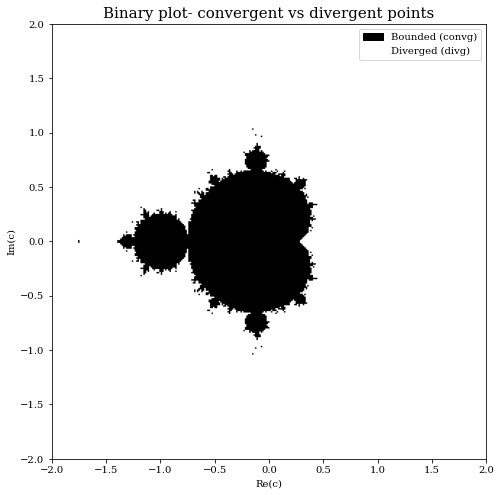
\includegraphics[scale=.4]{A3_q1_binary.png}}
\caption{Binary complex points map. Points in the sequence that diverge are white, points that converge are black.}
\label{fig}
\end{figure}

\begin{figure}[htbp]
\centerline{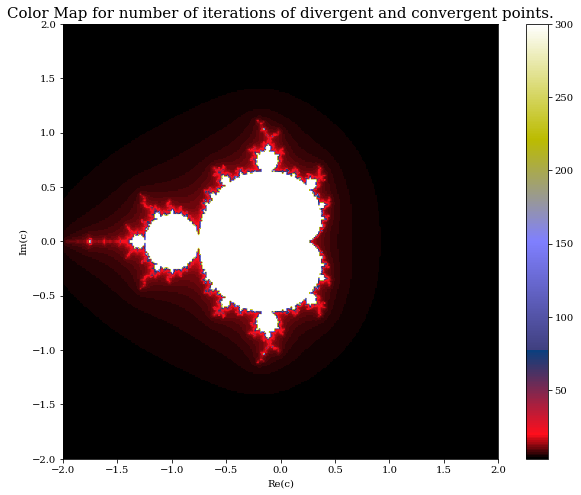
\includegraphics[scale=.4]{A3_q1_iter.png}}
\caption{Colorscale map with colorscale indicating the number of iterations of the sequence before the divergence of the point.}
\label{fig}
\end{figure}

\newpage
\section{Question 2}
\subsection{Methods}

In Python, I first defined a function my\_lorentz to code the differential equations. To solve them, solve\_ivp from scipy was used to numerically integrate the equations over a 60s period using the respective initial conditions and parameters. Specifically the Runge-Kutta method was used, as inputed in solve\_ivp as 'RK45'. The input t\_eval was of length 1000 to ensure enough solutions were computed.  \newline

To reproduce Lorenz's Figure 1 (Figure 3 in this document), matplotlib.pyplot was used to visualize the data. Each segment of the solution $Y(t)$ in the differential equation was plotted for different time steps $N=\frac{t}{\Delta t}$, each being 1000 units in length. These graphs are plotted on 3 subplots of the same figure. The top-most plot for the first 1000 time steps, the second for the time steps 1000-2000, and lastly the third for that of 2000-3000. The results are consistent with Lorenz's Figure 1. \newline

The reproduction of Figure 2 (Z-Y phase space plane) was done by plotting the solutions to the $Z(t)$ and $Y(t)$ equations against each other. This is seen in Figure 4 of this document. They are consistent with Lorenz's figure, showcasing the segment of the trajectory corresponding to the 1400-1900th iterations. In the function solve\_ivp, denseoutput=True was set to ensure that a continuous function was built over the t\_evals span. Consequently, this allows sol.sol(t\_evals) to evaluate the solutions of the differential equations for each point in t\_evals from the continuous distribution that was computed. Similarly, for the X-Y phase space plane, the solutions to the $X(t)$ and the $Y(t)$ differential equations were plotted against each other. They are also consistent with Lorenz's figure. \newline

To produce the last figure displaying the differences between both solutions as a function of time (Figure 5), first I computed the difference between the two solution arrays using list comprehension. This was done to obtain the space separation of each point (in 3D) at each time point. Next, given that the shape of this array was (3, 1000), the tranpose was taken for simplicity of working with time as the main vertical axis for each column of solutions $x(t), y(t) , z(t)$. Next, using np.lingalg.norm() the euclidean norm between each set of points was computed and stored in an array of shape (1000,). The results were plotted with a semilog yscale axis and a regular time axis (in seconds) with limits (0,60) and 1000 time steps. The result is an oscillating curve with a linear trend resembling a straight line. A linear model was fit to the data for the given time interval exhibiting a linear trend to visualize this aspect. 
\newpage
\subsection{Results}
% \begin{figure}[htbp]
%     \centering
%     \begin{subcaption}{0.38\textwidth}
%         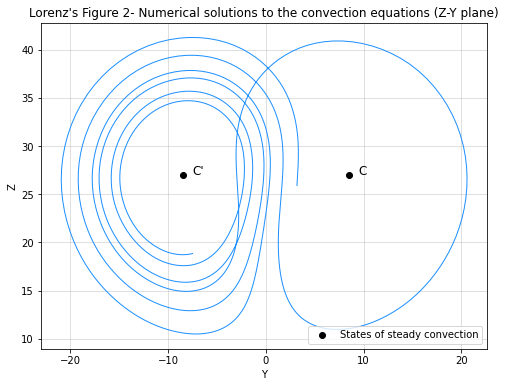
\includegraphics[width=\linewidth]{A3_q2_2_1.png}
%         \caption{Lorenz's Figure 2- upper plot. The numerical solutions to the convection equations projected on the Z-Y plane.}
%     \end{subcaption}
%     \hfill
%     \begin{subcaption}{0.38\textwidth}
%         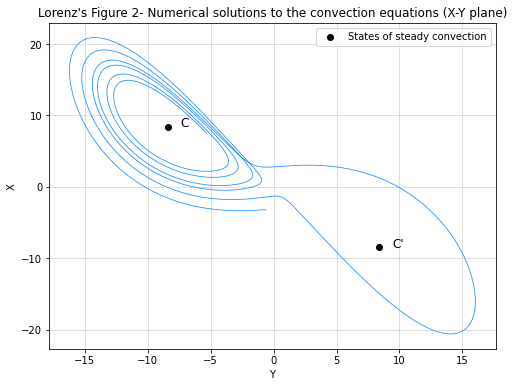
\includegraphics[width=\linewidth]{A3_q2_3_1.png}
%         \caption{Lorenz's Figure 2- lower plot. The numerical solutions to the convection equations projected on the X-Y plane.}
%     \end{subcaption}
%     \caption{Lorenz's Figure 2, numerical solutions to the convection equations. Figure (a) showcases the solutions in the Z-Y plane. Figure (b) displays the solutions in the X-Y plane.}
% \end{figure}

\begin{figure}[htbp]
\centerline{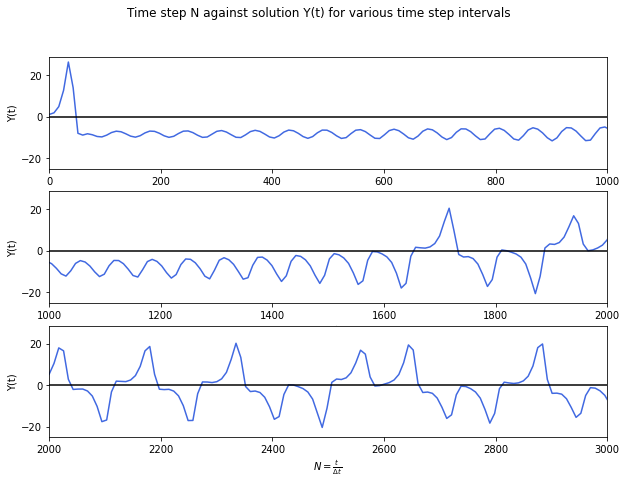
\includegraphics[scale=.5]{A3_q2_plot1_1.png}}
\caption{Lorenz's Figure 1 reproduced using appropriate initial conditions and parameters as specified.}
\label{fig}
\end{figure}

\begin{figure}[htbp]
\centerline{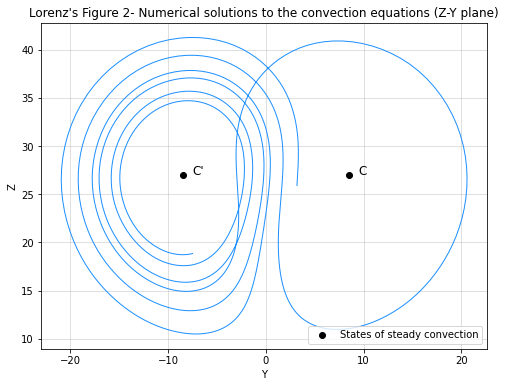
\includegraphics[scale=.6]{A3_q2_2_1.png}}
\caption{Lorenz's Figure 2- upper plot. The numerical solutions to the convection equations projected on the Z-Y plane.}
\label{fig}
\end{figure}

\begin{figure}[htbp]
\centerline{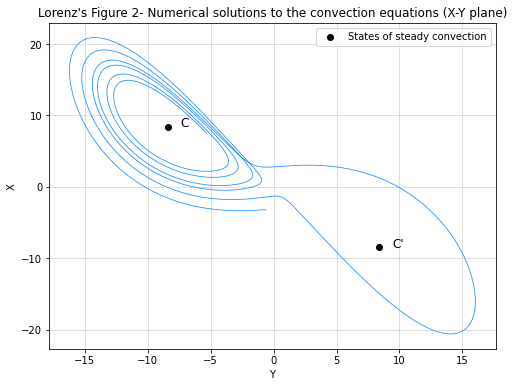
\includegraphics[scale=.6]{A3_q2_3_1.png}}
\caption{Lorenz's Figure 2- lower plot. The numerical solutions to the convection equations projected on the X-Y plane.}
\label{fig}
\end{figure}

\begin{figure}[htbp]
\centerline{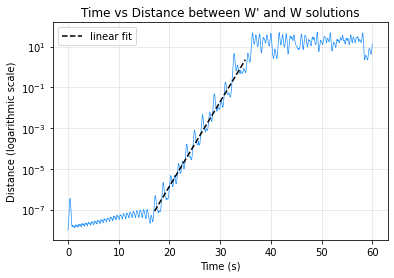
\includegraphics[scale=.8]{A3_q2_4_1.png}}
\caption{The distance between W' and W\_0 plotted as a function of time. Semilog y-axis to showcase the quasi-linear trend consistent with Lorenz's results.}
\label{fig}
\end{figure}

\end{document}
